\documentclass{article}
\usepackage[UTF8]{ctex}
\usepackage{amsmath,amssymb}
\usepackage{geometry}
\usepackage{graphicx}
\usepackage{booktabs}
\usepackage{multirow}
\usepackage{caption}
\usepackage{float}
\usepackage{gensymb}
\usepackage{diagbox}
\geometry{left=2cm,right=2cm,top=2cm,bottom=2cm}
\numberwithin{equation}{section}
\numberwithin{table}{section}
\setlength{\abovecaptionskip}{5pt}
\title{计算物理学作业2}
\author{庄铖}
\begin{document}
\maketitle
\section{多项式插值}
\subsection{5个等距节点}
利用Neville插值,可以得到插值后的函数。Neville插值的代码在na.py当中(na.py会随作业次数逐渐更新)。
得到
\begin{align}
    f\left(x\right)=0.996317 x + 0.0199514 x^2 - 0.203585 x^3 + 0.0287142 x^4
\end{align}
最大可能误差为
\begin{align}
    \frac{\left|x_n-x_0\right|^{n+1}}{\left(n+1\right)!}=0.08
\end{align}
\subsection{验证插值}
随机选择5个点:
$$1.500,0.728,0.379,1.142,0.939$$
计算得到$f\left(x\right)$的值为:
$$0.9976,0.6654,0.3700,0.9094,0.8069$$
函数$sin\left(x\right)$的值为:
$$0.9975,0.6654,0.3700,0.9095,0.8070$$
可见所有误差均远小于误差最大值。
\subsection{节点数估计}
若按照最大误差(很保守)来估计,则有:
\begin{align}
    \frac{\left|x_n-x_0\right|^{n+1}}{\left(n+1\right)!} & <10^{-8} \\
    n                                                    & =14
\end{align}
若按照实际误差来看,可以得到
\begin{align}
    n=9
\end{align}
此时最大误差约为$4\times10^{-9}$。本题所有代码可见1.py。
\section{Runge效应}
为了使pdf页数少一点,直接把三个小问都打出来了。
\begin{table}[H]
    \centering
    \caption{各种插值函数之间的比较}
    \scalebox{0.8}{
        \begin{tabular}{cccccccc}
            \toprule
            $point$ & $f(x)$   & $P20(x)$   & $fT(x)$  & $fC(x)$  & $P20(x)-f(x)$ & $fT(x)-f(x)$ & $fC(x)-f(x)$ \\
            \midrule
            0       & 0.038462 & 0.038462   & 0.038691 & 0.038708 & 0.000000      & 0.000000     & 0.000000     \\
            1       & 0.042440 & -39.952449 & 0.041012 & 0.039691 & 39.994889     & 0.001390     & 0.000094     \\
            2       & 0.047059 & 0.047059   & 0.040588 & 0.040683 & 0.000000      & 0.000000     & 0.000000     \\
            3       & 0.052459 & 3.454958   & 0.041028 & 0.042693 & 3.402499      & 0.001573     & 0.000028     \\
            4       & 0.058824 & 0.058824   & 0.044765 & 0.044813 & 0.000000      & 0.000000     & 0.000000     \\
            5       & 0.066390 & -0.447052  & 0.050051 & 0.048235 & 0.513442      & 0.001801     & 0.000004     \\
            6       & 0.075472 & 0.075472   & 0.052152 & 0.052123 & 0.000000      & 0.000000     & 0.000000     \\
            7       & 0.086486 & 0.202423   & 0.055761 & 0.057928 & 0.115936      & 0.002170     & 0.000013     \\
            8       & 0.100000 & 0.100000   & 0.064702 & 0.064707 & 0.000000      & 0.000000     & 0.000000     \\
            9       & 0.116788 & 0.080660   & 0.077294 & 0.074500 & 0.036128      & 0.002795     & 0.000001     \\
            10      & 0.137931 & 0.137931   & 0.086621 & 0.086608 & 0.000000      & 0.000000     & 0.000000     \\
            11      & 0.164948 & 0.179763   & 0.100421 & 0.104338 & 0.014814      & 0.003918     & 0.000084     \\
            12      & 0.200000 & 0.200000   & 0.127794 & 0.127802 & 0.000000      & 0.000000     & 0.000000     \\
            13      & 0.246154 & 0.238446   & 0.169511 & 0.163290 & 0.007708      & 0.006138     & 0.000114     \\
            14      & 0.307692 & 0.307692   & 0.214539 & 0.214577 & 0.000000      & 0.000000     & 0.000000     \\
            15      & 0.390244 & 0.395093   & 0.285364 & 0.296582 & 0.004849      & 0.011144     & 0.000824     \\
            16      & 0.500000 & 0.500000   & 0.423295 & 0.422375 & 0.000000      & 0.000000     & 0.000000     \\
            17      & 0.640000 & 0.636755   & 0.645255 & 0.624928 & 0.003245      & 0.023376     & 0.003169     \\
            18      & 0.800000 & 0.800000   & 0.866629 & 0.865072 & 0.000000      & 0.000000     & 0.000000     \\
            19      & 0.941176 & 0.942490   & 0.962410 & 1.000000 & 0.001314      & 0.037590     & 0.002310     \\
            20      & 1.000000 & 1.000000   & 0.866629 & 0.865072 & 0.000000      & 0.000000     & 0.000000     \\
            21      & 0.941176 & 0.942490   & 0.645255 & 0.624928 & 0.001314      & 0.023376     & 0.002310     \\
            22      & 0.800000 & 0.800000   & 0.423295 & 0.422375 & 0.000000      & 0.000000     & 0.000000     \\
            23      & 0.640000 & 0.636755   & 0.285364 & 0.296582 & 0.003245      & 0.011144     & 0.003169     \\
            24      & 0.500000 & 0.500000   & 0.214539 & 0.214577 & 0.000000      & 0.000000     & 0.000000     \\
            25      & 0.390244 & 0.395093   & 0.169511 & 0.163290 & 0.004849      & 0.006138     & 0.000824     \\
            26      & 0.307692 & 0.307692   & 0.127794 & 0.127802 & 0.000000      & 0.000000     & 0.000000     \\
            27      & 0.246154 & 0.238446   & 0.100421 & 0.104338 & 0.007708      & 0.003918     & 0.000114     \\
            28      & 0.200000 & 0.200000   & 0.086621 & 0.086608 & 0.000000      & 0.000000     & 0.000000     \\
            29      & 0.164948 & 0.179763   & 0.077294 & 0.074500 & 0.014814      & 0.002795     & 0.000084     \\
            30      & 0.137931 & 0.137931   & 0.064702 & 0.064707 & 0.000000      & 0.000000     & 0.000000     \\
            31      & 0.116788 & 0.080660   & 0.055761 & 0.057928 & 0.036128      & 0.002170     & 0.000001     \\
            32      & 0.100000 & 0.100000   & 0.052152 & 0.052123 & 0.000000      & 0.000000     & 0.000000     \\
            33      & 0.086486 & 0.202423   & 0.050051 & 0.048235 & 0.115936      & 0.001801     & 0.000013     \\
            34      & 0.075472 & 0.075472   & 0.044765 & 0.044813 & 0.000000      & 0.000000     & 0.000000     \\
            35      & 0.066390 & -0.447052  & 0.041028 & 0.042693 & 0.513442      & 0.001573     & 0.000004     \\
            36      & 0.058824 & 0.058824   & 0.040588 & 0.040683 & 0.000000      & 0.000000     & 0.000000     \\
            37      & 0.052459 & 3.454958   & 0.041012 & 0.039691 & 3.402499      & 0.001390     & 0.000028     \\
            38      & 0.047059 & 0.047059   & 0.038691 & 0.038708 & 0.000000      & 0.000000     & 0.000000     \\
            39      & 0.042440 & -39.952449 & 0.962410 & 1.000000 & 39.994889     & -            & 0.000094     \\
            40      & 0.038462 & 0.038462   & 0.962410 & 1.000000 & 0.000000      & -            & 0.000000     \\
            \bottomrule
        \end{tabular}
    }
\end{table}
(1)问中的图:
\begin{figure}[H]
    \begin{minipage}[t]{0.48\linewidth}
        \centering
        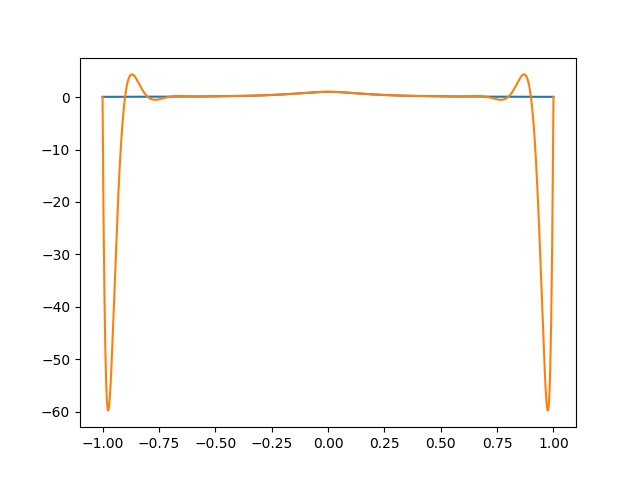
\includegraphics[scale=0.5]{P20.jpg}
        \caption{P20}
    \end{minipage}
    \begin{minipage}[t]{0.48\linewidth}
        \centering
        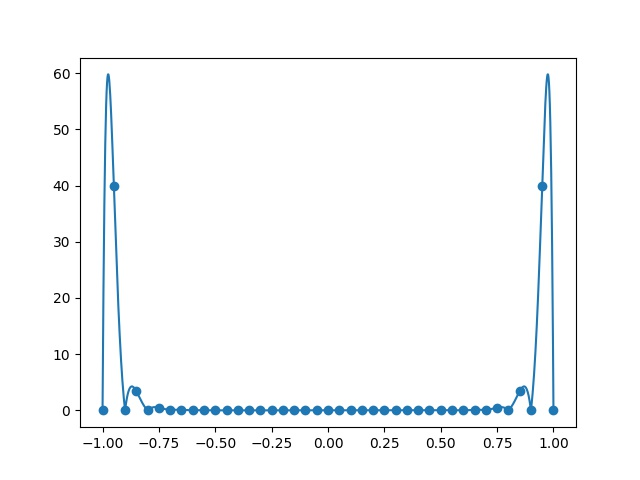
\includegraphics[scale=0.5]{P20.sub.jpg}
        \caption{P20误差}
    \end{minipage}
\end{figure}
\begin{figure}[H]
    \begin{minipage}[t]{0.48\linewidth}
        \centering
        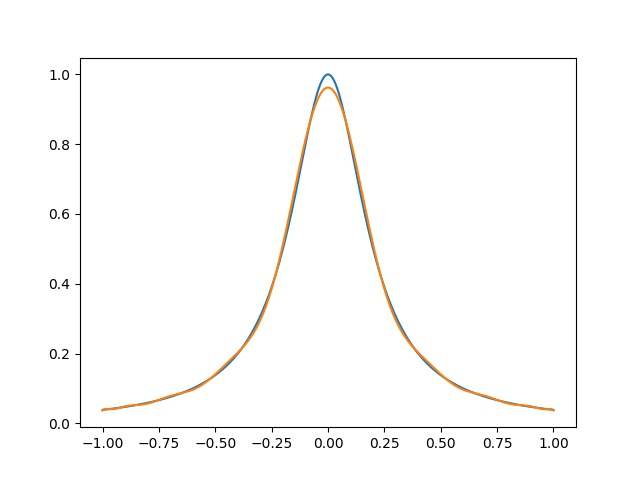
\includegraphics[scale=0.5]{fChebyshev.jpg}
        \caption{Chebyshev}
    \end{minipage}
    \begin{minipage}[t]{0.48\linewidth}
        \centering
        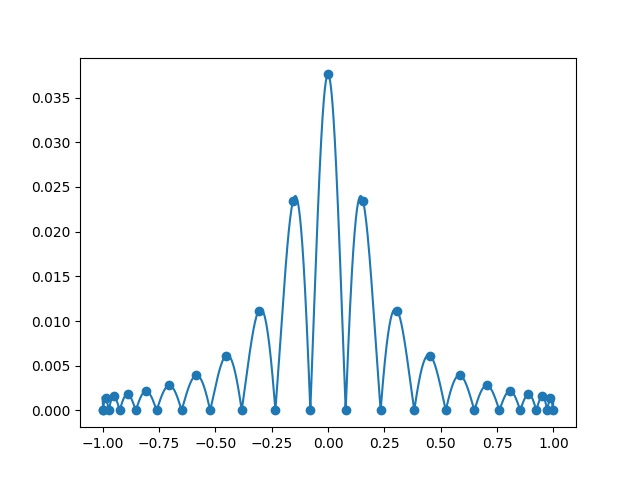
\includegraphics[scale=0.5]{fChebyshev.sub.jpg}
        \caption{Chebyshev误差}
    \end{minipage}
\end{figure}
\begin{figure}[H]
    \begin{minipage}[t]{0.48\linewidth}
        \centering
        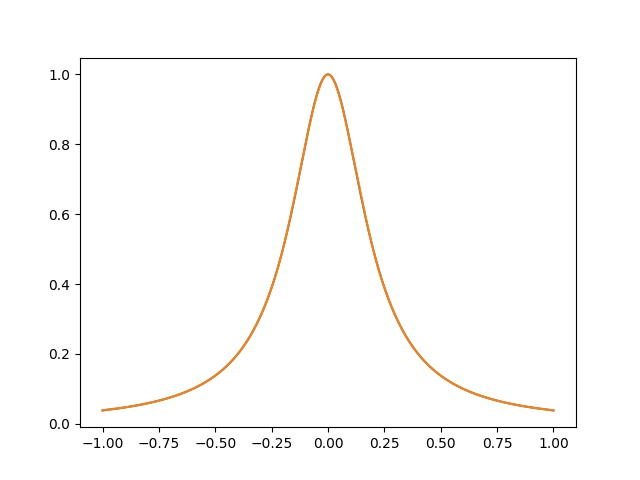
\includegraphics[scale=0.5]{fCubicSpline.jpg}
        \caption{CubicSpline}
    \end{minipage}
    \begin{minipage}[t]{0.48\linewidth}
        \centering
        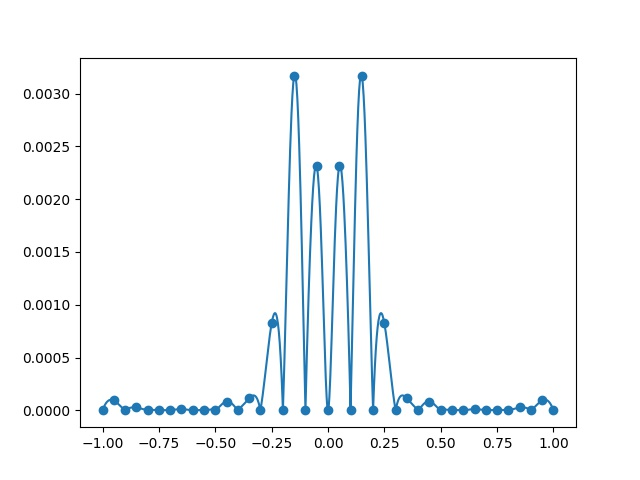
\includegraphics[scale=0.5]{fCubicSpline.sub.jpg}
        \caption{CubicSpline误差}
    \end{minipage}
\end{figure}
\section{样条函数在计算机绘图中的运用}
\subsection{选点列表}
\begin{table}[H]
    \centering
    \caption{$x_t$,$y_t$}
    \scalebox{0.9}{
        \begin{tabular}{cccccccccc}
            \toprule
            $t$   & 0        & 1        & 2        & 3         & 4         & 5         & 6         & 7         & 8         \\
            \midrule
            $x_t$ & 0.000000 & 0.207107 & 0.000000 & -1.207107 & -2.000000 & -1.207107 & -0.000000 & 0.207107  & 0.000000  \\
            $y_t$ & 0.000000 & 0.207107 & 1.000000 & 1.207107  & 0.000000  & -1.207107 & -1.000000 & -0.207107 & -0.000000 \\
            \bottomrule
        \end{tabular}
    }
\end{table}
\subsection{给出样条函数}
两个函数$S_\Delta\left(x;t\right)$,$S_\Delta\left(y;t\right)$均已在代码3.py中给出。选用周期边界条件。
\begin{table}[H]
    \centering
    \caption{x的系数}
    \begin{tabular}{ccccc}
        \toprule
        分段 & 0次     & 1次     & 2次    & 3次    \\
        \midrule
        0    & 0.000   & -0.000  & 0.690  & -0.451 \\
        1    & -0.045  & 0.171   & 0.472  & -0.358 \\
        2    & -4.045  & 7.811   & -4.392 & 0.674  \\
        3    & -2.835  & 6.270   & -3.738 & 0.581  \\
        4    & 33.221  & -28.161 & 7.222  & -0.581 \\
        5    & 38.823  & -32.441 & 8.312  & -0.674 \\
        6    & -69.177 & 36.314  & -6.279 & 0.358  \\
        7    & -84.548 & 44.702  & -7.804 & 0.451  \\
        \bottomrule
    \end{tabular}
\end{table}
\begin{table}[H]
    \centering
    \caption{y的系数}
    \begin{tabular}{ccccc}
        \toprule
        分段 & 0次     & 1次     & 2次    & 3次    \\
        \midrule
        0    & 0.000   & 0.043   & -0.000 & 0.358  \\
        1    & 0.455   & -1.696  & 2.214  & -0.581 \\
        2    & -0.052  & -0.728  & 1.597  & -0.451 \\
        3    & -14.762 & 18.002  & -6.352 & 0.674  \\
        4    & -14.762 & 18.002  & -6.352 & 0.674  \\
        5    & 53.340  & -34.024 & 6.897  & -0.451 \\
        6    & 67.030  & -42.739 & 8.746  & -0.581 \\
        7    & -89.098 & 42.456  & -6.750 & 0.358  \\
        \bottomrule
    \end{tabular}
\end{table}
\subsection{画图并比较}
作图如下。
\begin{figure}[H]
    \centering
    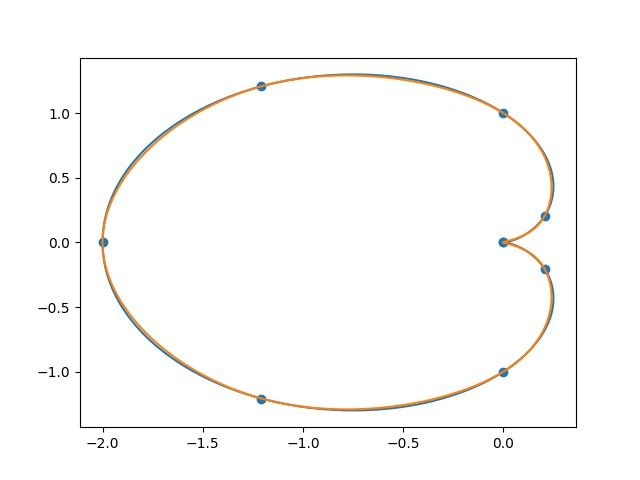
\includegraphics[scale=0.5]{cardioid.jpg}
    \caption{内插与原先心形线}
\end{figure}
\subsection{简要说明}
对于函数$f\left(x,y\right)=0$,有
\begin{align}
    \frac{\mathrm{d}y}{\mathrm{d}x}     & =\frac{y^\prime\left(t\right)}{x^\prime\left(t\right)}                                                                                      \\
    \frac{\mathrm{d}^2y}{\mathrm{d}x^2} & =\frac{y^{\prime\prime}\left(t\right)x^\prime\left(t\right)-y^\prime\left(t\right)x^{\prime\prime}\left(t\right)}{x^\prime\left(t\right)^3} \\
    \rho                                & =\frac{\left|y^{\prime\prime}\left(x\right)\right|}{\left(y^\prime\left(x\right)^2+1\right)^{\frac{3}{2}}}
\end{align}
因此在节点处一阶导,二阶导以及曲率半径都连续,看起来很光滑。
\section{计算积分}
\begin{align}
    \int_{-\infty}^\infty e^{-x^2}cos\left(x\right)=\sqrt{\pi}e^{-\frac{1}{4}}=1.380388447043143
\end{align}
\subsection{梯形法}
利用na.py中Integrate函数选项method="ladder",可以得到
\begin{table}[H]
    \centering
    \caption{不同区间与步长求得的积分值}
    \begin{tabular}{c|cccc}
        \diagbox{区间}{分割} & $10^2$             & $10^3$             & $10^4$             & $10^5$             \\
        \hline
        $\pm1$               & 1.3123482540682647 & 1.3123482540682647 & 1.3123482540682647 & 1.3123482540682647 \\
        $\pm5$               & 1.3803884470421277 & 1.3803884470421277 & 1.3803884470421277 & 1.3803884470421277 \\
        $\pm10$              & 1.3803884470431431 & 1.3803884470431431 & 1.3803884470431431 & 1.3803884470431431 \\
        $\pm15$              & 1.3803884470431427 & 1.3803884470431427 & 1.3803884470431427 & 1.3803884470431427 \\
    \end{tabular}
\end{table}
可见当区间较大且分割块数较多时非常接近于精确值。
\subsection{外推积分法}
利用na.py中Integrate函数选项method="extrapolation",可以得到
\begin{table}[H]
    \centering
    \caption{不同区间与步长求得的积分值}
    \begin{tabular}{c|ccccc}
        \diagbox{区间}{m} & $14$               & $15$               & $16$               & $17$               \\
        \hline
        $\pm1$            & 1.3123487254630597 & 1.3123487254629609 & 1.3123487254630417 & 1.3123487254630148 \\
        $\pm5$            & 1.3803884470421155 & 1.3803884470422174 & 1.3803884470420744 & 1.3803884470417724 \\
        $\pm10$           & 1.3803884470431027 & 1.3803884470431012 & 1.380388447043165  & 1.380388447042966  \\
        $\pm15$           & 1.3803884470431462 & 1.3803884470431014 & 1.3803884470431131 & 1.3803884470430943 \\
    \end{tabular}
\end{table}
可见外推法离精确值仍差几个机器精度,而$2^{17}=131072>10^5$因此外推法在这里不如梯形(
\subsection{高斯积分法}
代码仍见4.py。
\begin{table}[H]
    \centering
    \caption{高斯积分法}
    \begin{tabular}{ccccc}
        \toprule
        $n$ & 5                  & 10                 & 15                 & 20                \\
        \midrule
        $T$ & 1.3803900759356564 & 1.3803884470431405 & 1.3803884470431425 & 1.380388447043143 \\
        \bottomrule
    \end{tabular}
\end{table}
可见当$n=20$时已经到达机器精度。
\end{document}